\lab{Applications}{Voronoi Diagrams and Delaunay Triangulations}{Voronoi Diagrams and Delaunay Triangulations}
\label{lab:voronoi}

\objective{Introduce Voronoid Diagrams and Delaunay Triangulations and discuss their applications}

\section*{Voronoi Diagrams}

In this lab we will discuss some applications of Voronoi Diagrams.
In the abstract sense, a Voronoi diagram is a partition of a plane into regions that lie closest to different points.
The easiest way to understand this is to look at some examples.
Figure \ref{voronoi_ex_1} is a voronoi diagram generated from 100 random points with $x$ and $y$ values between 0 and 1.
Notice how each point has a small  cell around it that is made up of the points that lie closest to it.

\begin{figure}
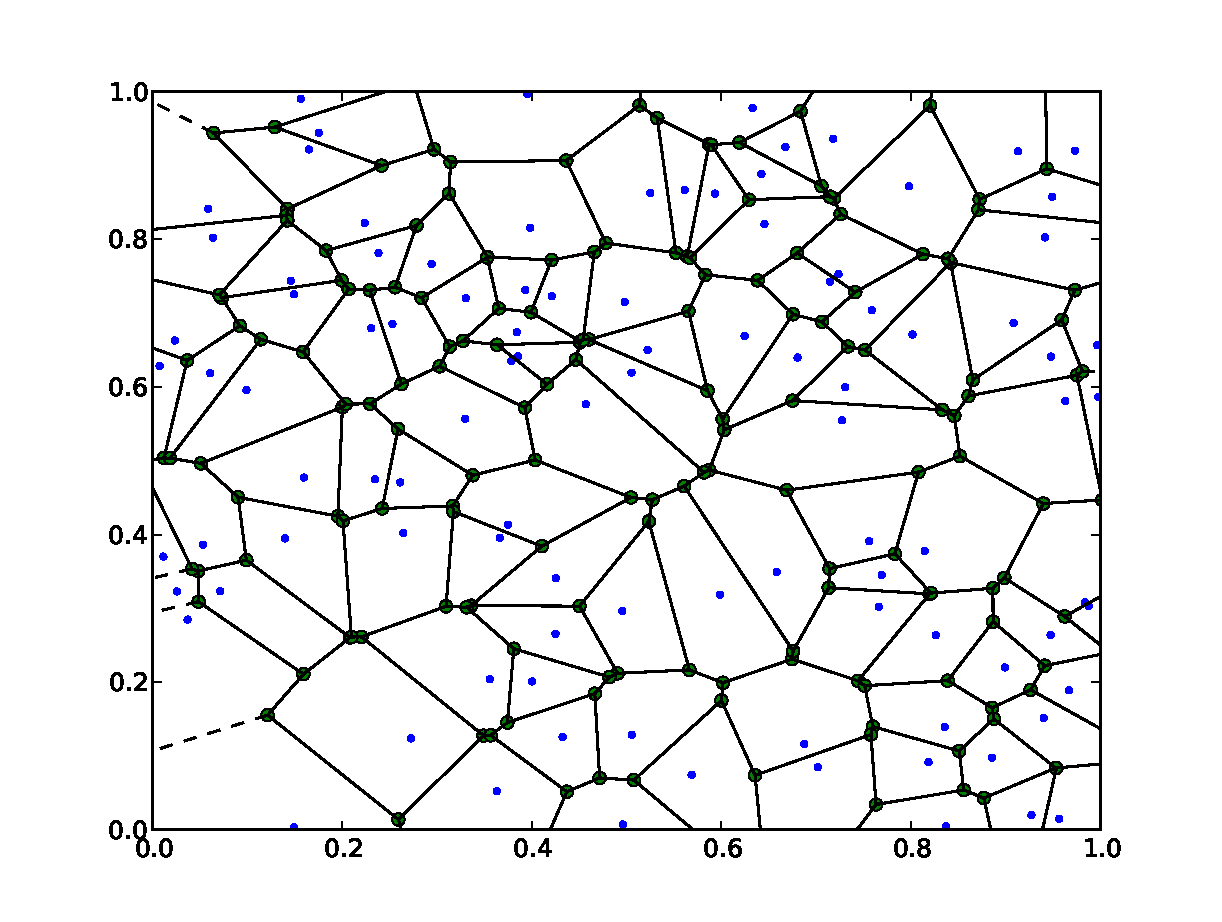
\includegraphics[width=\textwidth]{voronoi_example_1.pdf}
\caption{A Voronoi diagram of the square $[0,1]\times [0,1]$ for 100 randomly generated points.}
\label{voronoi_ex_1}
\end{figure}

One possible way to compute this sort of diagram would be by brute force, for example:
\begin{lstlisting}
import numpy as np
from numpy.random import rand
from matplotlib imort pyplot as plt
num = 10
res = 201
pts = rand(num, 2)
X = np.linspace(0, 1, res)
Y = X.copy()
X, Y = np.meshgrid(X, Y)
Z = np.empty_like(X)
indices = np.zeros_like(X)
for i in xrange(res):
    for j in xrange(res):
        #note: we don't need to do the sqare root
        #since we really just need to compare the distances
        mn = (X[i,j] - pts[0,0])**2 + (Y[i,j] - pts[0,1])**2
        for k in xrange(1,num):
            dist = (X[i,j] - pts[k,0])**2 + (Y[i,j] - pts[k,1])**2
            if dist < mn:
                indices[i,j] = k
                mn = dist
plt.pcolormesh(X,Y,indices)
plt.scatter(pts[:,0],pts[:,1])
plt.xlim((0,1))
plt.ylim((0,1))
plt.show()
\end{lstlisting}
This algorithm is good because it can work regardless of the metric space we are using, but it is terribly slow.
Figure \ref{voronoi_1norm} shows a similar diagram using the 1-norm and figure \ref{voronoi_supnorm} shows a diagram generated using the supremum norm.
It is linear in the number of points added and linear in the number of pixels used to represent the diagram.
This can be a terrible limitation, but if you are not working in a well behaved metric space, this may be the simplest approach.
\begin{figure}
\begin{minipage}[b]{0.45\linewidth}
\centering
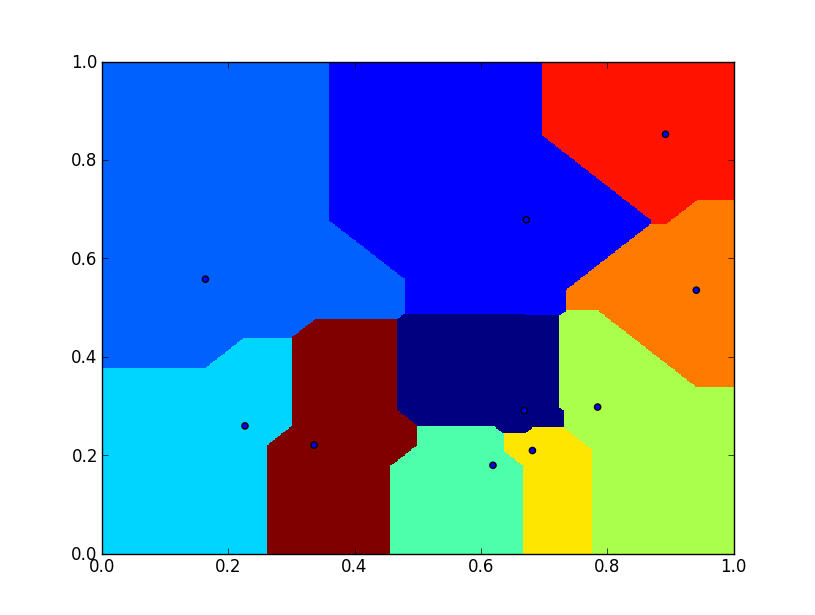
\includegraphics[width=\textwidth]{voronoi_1norm.png}
\caption{Voronoi diagram in the 1-norm}
\label{voronoi_1norm}
\end{minipage}
\hspace{0.5cm}
\begin{minipage}[b]{0.45\linewidth}
\centering
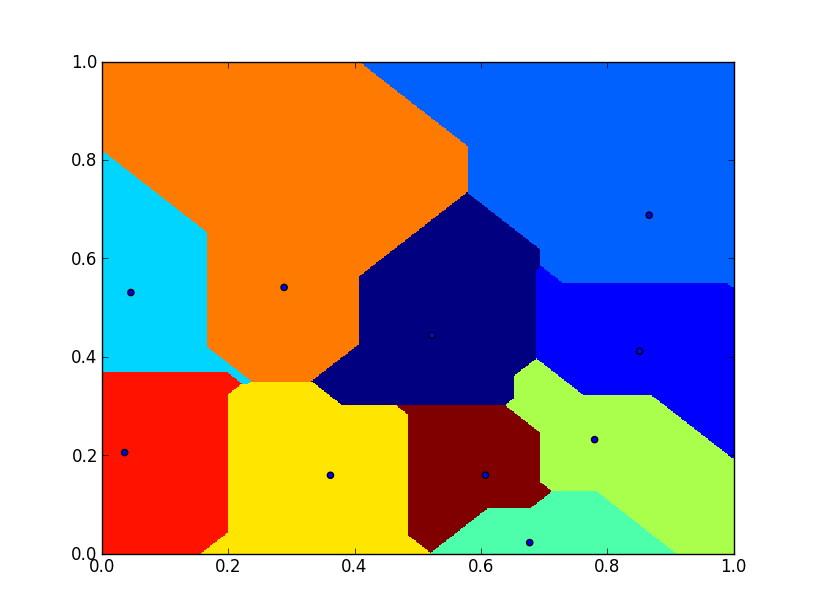
\includegraphics[width=\textwidth]{voronoi_supnorm.png}
\caption{Voronoi diagram in the supremum norm}
\label{voronoi_supnorm}
\end{minipage}
\end{figure}

There are several data structures used in the field of computational geometry that can store the exact edges of diagrams like this.
We would prefer to not have to worry about sampling the domain in this way.
There are a variety of algorithms that can compute Voronoi diagrams in $\mathcal{O}\left( n \log\left(n\right)\right)$ time (where $n$ is the number of points).
Fortune's algorithm is a linesweep algorithm that can do this.
SciPy includes a wrapper of the Qhull library which includes an algorithm to compute voronoi diagrams based on convex hulls.

A plot similar to the one we just generated can be made using SciPy like this:
\begin{lstlisting}
import numpy as np
from numpy.random import rand
import scipy.spatial as st
from matplotlib import pyplot as plt
G = rand(100,2)
G = st.Voronoi(G)
st.voronoi_plot_2d(G)
plt.xlim((0, 1))
plt.ylim((0, 1))
plt.show()
\end{lstlisting}
Notice how much clearer the plot is and how much faster it is generated.
Try running the last bit of code for 1000 points.
Though this is a little slower than it was for 10 points, this is a graph that would not display well if we had been using the brute force method.

%intro scipy.spatial implementation. teach the different methods available.
%Be sure to mention KDTrees so they can try a few different implementations of the problems.

\section*{Applications of Voronoi Diagrams}

%Tell the John snow cholera story

%problem using voronoi diagrams as a basis for nearest neighbor queries

%Taxi service problem, Lifelight example

%Retail store placement problem

%Estimate ore deposits and rainfall

\section*{Delaunay Triangulation}

%Mention FEM triangulation and have them write some basic code for it.

\section*{Applications of Delaunay Triangulations}

%Use Delaunay Triangulation to tesselate a 3d surface.
%Use tesselation to rerun ore/rainfall problem and compare results.